\newpage
\section{Programacion lineal entera}

En este trabajo se opt\'o por reducir el problema a un problema de conjunto independiente de peso m\'aximo en un grafo dado por la discretizaci\'on del \'area del yacimiento, que proporcion\'o buenos resultados en la pr\'actica. Dado un grafo $G=(V,E)$, un \textbf{conjunto independiente} es un conjunto $I\subseteq V$ de v\'ertices tal que $ij\not\in E$ para todo $i,j\in I$. Si adem\'as tenemos una funci\'on de peso W : V $\rightarrow \mathbb{R}$, el \textbf{peso} del conjunto independiente $I$ es $w(I) := \sum_{i\in I} w_i$. La motivaci\'on para este enfoque viene dada por el hecho de que el conjunto de pads de la soluci\'on conforma un conjunto de elementos no conflictivos entre s\'\i, situaci\'on que es modelada adecuadamente por medio de conjuntos independientes en un grafo. Sin embargo, esta reducci\'on trae aparejado un \emph{costo de discretizaci\'on}, que ser\'a mayor cuanto mayor sea el paso de discretizaci\'on seleccionado.

A grandes rasgos, el algoritmo propuesto est\'a compuesto por los siguientes puntos:
\begin{enumerate}
\item Discretizaci\'on $D\subseteq Y$ del \'area geogr\'afica del yacimiento.
\item Generaci\'on de un conjunto $T$ de pads posibles sobre la base de la discretizaci\'on $D$.
\item Planteo de un grafo $G=(T,E)$, de modo tal que cada conjunto independiente de $G$ corresponde a una soluci\'on factible del problema de optimizaci\'on del \'area de drenaje. Los v\'ertices del grafo reciben pesos adecuadamente definidos, de modo tal que el peso de cada conjunto independiente corresponde a la funci\'on objetivo de la soluci\'on factible.
\item B\'usqueda de un conjunto independiente de peso m\'aximo sobre $G$ por medio de un modelo de programaci\'on lineal entera, para obtener una soluci\'on $P$ al problema.
\end{enumerate}
Describimos a continuaci\'on cada punto del algoritmo. Para esto, sean $\Delta_x$, $\Delta_y$ $\in$ $\mathbb{R}_{+}$ los \textbf{pasos de discretizaci\'on} y sea $A=\{\alpha_1,\dots,\alpha_p\}$ un conjunto de \'angulos posibles, de modo tal que $\alpha_i\in[\alpha-\beta,\alpha+\beta]$ para $i=1,\dots,p$. En nuestra implementaci\'on computacional, tomamos $A=\{\alpha-\beta,\alpha,\alpha+\beta\}$.


\noindent\textbf{Discretizaci\'on.} El primer paso del algoritmo consiste en generar una discretizaci\'on $D=\{(x_i,y_i)\}_{i=1}^m$ por filas y columnas del \'area del yacimiento, de modo tal que dos puntos consecutivos de una misma fila est\'en a distancia $\Delta_x$ y dos puntos consecutivos de una misma columna est\'en a distancia $\Delta_y$. Para esto, se genera un reticulado de puntos en el plano con \'angulo $\alpha$.


\noindent\textbf{Generaci\'on de pads.} Para cada punto $(x,y)\in D$ de la discretizaci\'on, cada configuraci\'on $S\in\S$ y cada \'angulo $i\in\{1,\dots,p\}$, se incluye en el conjunto $T$ un pad $P$ con configuraci\'on $S$, centrado en $(x,y)$ y rotado en \'angulo $\alpha_i$, siempre que el pad $P$ (i) est\'e incluido completamente dentro de $Y$ y (ii) su locaci\'on $L$ no interseque con ning\'un obst\'aculo. Para determinar este \'ultimo punto, se consideran como centros posibles de la locaci\'on el punto $(x,y)$ y ocho puntos equiangulados sobre la circunferencia de centro $(x,y)$ y radio $tol_S$, y se considera que se cumple la condici\'on (ii) si para alguno de estos puntos, la locaci\'on centrada en ese punto no interseca a ning\'un obst\'aculo. Este enfoque es arbitrario e incurre en un nuevo error de discretizaci\'on, pero se observ\'o que genera resultados aceptables en la pr\'actica.


\noindent\textbf{Grafo de conflictos.} Se genera un grafo $G=(T,E)$ cuyos v\'ertices est\'an dados por todos los pads generados en el punto anterior, y cuyas aristas unen pares de pads con intersecci\'on no vac\'\i a. El conjunto $E$ est\'a compuesto por los pares $(P_1,P_2)$ tales que existe alg\'un punto $(x,y)\in D$ con $(x,y)\in P_1$ y $(x,y)\in P_2$. Esta definici\'on de $E$ permite que existan pares de pads con peque\~nas superposiciones pero sin una arista que los una en $G$. Esto sucede cuando la intersecci\'on no contiene ning\'un punto de la discretizaci\'on $D$, lo cual puede ocurrir s\'olo cuando la superposici\'on es peque\~na. De este modo, se maneja adecuadamente la restricci\'on el\'astica de no superposici\'on de pads.

\noindent\textbf{Obtenci\'on de una soluci\'on.} Se plantea y se resuelve la siguiente formulaci\'on de conjunto independiente con peso m\'aximo sobre $G$, usando las restricciones clique sobre todos los puntos de la discretizaci\'on. En este modelo, se tiene una variable binaria $x_P$ por cada pad, de modo tal que $x_P=1$ si y s\'olo si el pad $P$ se incluye en la soluci\'on.


\begin{center}
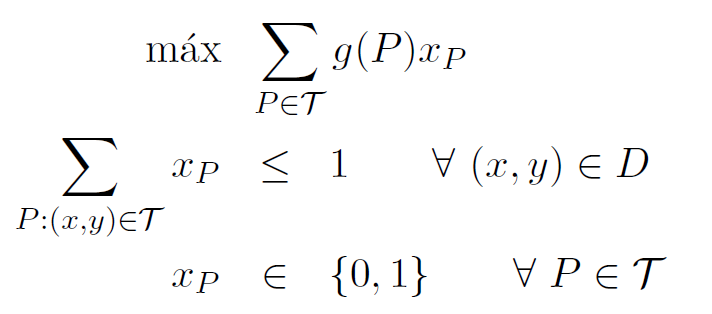
\includegraphics[width=0.5\textwidth]{imagenes/formula}
\end{center}




El coeficiente $g(P)$ asociado con la variable $x_P$ en la funci\'on objetivo es $g(P) = neto(P)$ si se optimiza el beneficio total (dado por la venta de la producci\'on total esperada menos los costos de construcci\'on), o bien $g(P) = area(P)$ si se optimiza el \'area total cubierta. 
Dado que los puntos de la discretizaci\'on $D$ generan todas las cliques maximales de $G$ (aunque no todo punto de $D$ genera necesariamente una clique maximal), esta formulaci\'on incluye todas las restricciones de la formulaci\'on por cliques del problema de conjunto independiente de peso m\'aximo, y se espera que sea m\'as fuerte que una formulaci\'on con una restricci\'on por arista. Dadas las caracter\'\i sticas aproximadas del procedimiento, no resulta imprescindible en la pr\'actica resolver en forma \'optima el modelo de programaci\'on entera planteado, aunque la pr\'oxima secci\'on muestra que en general este modelo se resuelve en forma exacta para tama\~nos de instancia razonables.

La generaci\'on de la discretizaci\'on $D$ es un paso clave dentro del algoritmo. Si los pasos de discretizaci\'on $\Delta_x$ y $\Delta_y$ son demasiado grandes, entonces no se generar\'a un n\'umero suficientemente grande y variado de pads en $T$ y la soluci\'on ser\'a de peor calidad, adem\'as de incluir potencialmente superposiciones entre los pads seleccionados, dado el modo en el que se generan las aristas de $G$. Sin embargo, a medida que $\Delta_x$ y $\Delta_y$ disminuyen se espera que estos efectos se vean minimizados, y que caigan por debajo de los errores de mediciones y de los par\'ametros de seguridad habituales en la industria hidrocarbur\'\i fera. A medida que  tienden a cero, la soluci\'on generada por este procedimiento tiende a la soluci\'on \'optima. Los experimentos computacionales presentados en la pr\'oxima secci\'on muestran que eligiendo adecuadamente los valores de $\Delta_x$ y $\Delta_y$ se obtienen buenos resultados.
